{
{\Large {\bfseries I}nfrared {\bfseries R}adiation (IR)}
\begin{itemize}

\item IR is sensed by humans as heat and is below the range of human vision. All creatures emit IR, and snakes can detect it.

\item IR remote control signals are invisible to the human eye but can be detected by some electronic cameras.

\newlength{\nIRdogHeight}   \setlength{\nIRdogHeight}{0.88in}
\item
\begin{tabular}[t]{@{}ll@{\hspace{0.05in}}r}
\raisebox{-.43\nIRdogHeight}{
	\begin{minipage}{.73in}
		{
			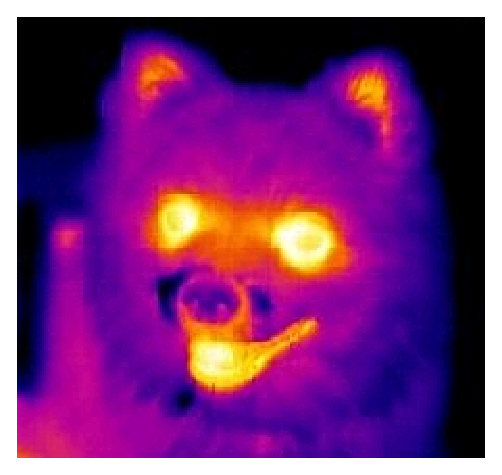
\includegraphics[height=\nIRdogHeight]{pictures/Infrared_dog.eps}
			\rput[b](-.4in,-.16in){\textcolor{gray}{\footnotesize\ NASA/IPAC}}
		}
	\end{minipage}
}&
 \begin{minipage}[t]{1.4in}Night vision scopes/goggles use a special camera that senses IR and converts the image to visible light. Some IR cameras employ an IR lamp to help illuminate the view.\end{minipage}&
 %
 % Get a regular outdoor night time photo with flash, use GIMP->Filters->EG-> Infrared Simulation
\raisebox{-.43\nIRdogHeight}{\
	\begin{minipage}{1in}
		{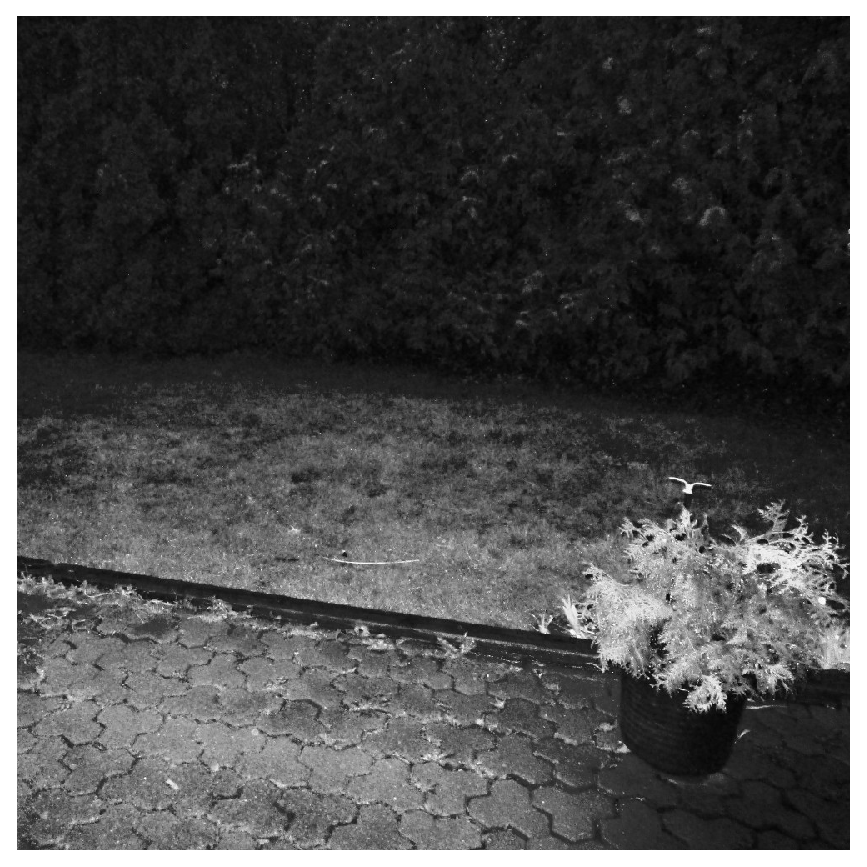
\includegraphics[height=\nIRdogHeight]{pictures/nightvision.eps}}
	\end{minipage}
}
\end{tabular}

\item A demonstration of IR is to hold a metal bowl in front of your face. The IR emitted by your body  will be reflected back using the parabolic shape of the bowl and you will feel the heat.

\item IR LASERs are used for cutting material.

%Information provided by Edward  Alan Dowdell:
%http://www.fiber-optics.info/fiber-history.htm
%http://www.thefoa.org/tech/wavelength.htm
%http://www.webopedia.com/TERM/E/EDFA.html
\item Fiber-optic based infrared communication signals are sometimes amplified with Erbium-Doped Fiber Amplifiers  \scalebox{.8}{\psframebox[linestyle=none]{\fiberoptics{0.13,-.13}{EDFA}}}
\end{itemize}
}
